%写在前面:
%建议首先阅读 README.txt
%本模版是【非官方】中央财经大学课程论文模版。因为使用本模版造成任何问题由使用者【自行承担】。

%注意:使用时,请使用XeLaTeX进行编译,不要用overleaf默认的pdfLaTeX进行编译。

%关于产权:
%本模版改编自:DoniaHakurei在GitHub的仓库中上传的模版(https://github.com/DoniaHakurei/CUFE_thesis_LaTeX_template)。原模版在某些地方,如封面的字体等不符合教务处最新要求,因此本人进行了相应修改。
%同时,本模版已经上传在本人的个人GitHub仓库中(个人主页:https://github.com/NathanHuXy)。
%作者:胡雪岩(金融科技20)
%邮箱:1033739554@qq.com

%请尊重作者产权。


%---------------------------------------------------------------------
%	个性化信息
%--------------------------------------------------------------------
\newcommand{\MYTITLE}{XXX策略研究}%论文标题
\newcommand{\MYID}{20xx310xxx}%学号
\newcommand{\MYNAME}{胡雪岩}%姓名
\newcommand{\MYCLASS}{Financial Technology}%班级
\newcommand{\MYADVISOR}{唐纳德·克努特}%任课教师
\newcommand{\MYCOURSE}{计算机程序设计的艺术}%课程名
\newcommand{\MYTERM}{1969-1973 第一学期}%学期
\newcommand{\MYCOURSEID}{20011021}%课程ID

%---------------------------------------------------------------------
%   各种导言
%--------------------------------------------------------------------
\documentclass[a4paper,12pt]{report}
\usepackage{geometry} % to change the page dimensions
\geometry{a4paper,left=2.5cm,right=2.5cm,top=2.54cm,bottom=2.54cm}%页边距
\usepackage{ctex}
\usepackage{xeCJK}
\usepackage{comment}
\usepackage{setspace}
\usepackage{fancyhdr}
\usepackage{graphicx}
\usepackage{wrapfig}
\usepackage{subfigure}
\usepackage{array}
\usepackage{titlesec}
\usepackage{titletoc}
\usepackage[titletoc]{appendix}
%\usepackage[top=30mm,bottom=30mm,left=20mm,right=20mm]{geometry}
%\usepackage{cite}

\setstretch{1.5}
%\usepackage{courier}
\setmonofont{Courier New}
\usepackage{listings}
%---------------------------------------------------------------------
%   参考文献设置
%--------------------------------------------------------------------
\usepackage[backend = biber, style = references/gb7714-2015, defernumbers=true]{biblatex}
\renewcommand*{\bibfont}{\small}
\addbibresource{references/bibs.bib}
\renewcommand{\bibname}{参考文献}
%---------------------------------------------------------------------
%	引用文献设置为上标
%---------------------------------------------------------------------
\begin{comment}
    \makeatletter
    \def\@cite#1#2{\textsuperscript{[{#1\if@tempswa , #2\fi}]}}
    \makeatother
\end{comment}

\lstset{tabsize=4, keepspaces=true,
    xleftmargin=2em,xrightmargin=0em, aboveskip=0.1em,
    %backgroundcolor=\color{gray!20},  % 定义背景颜色
    frame=none,                       % 表示不要边框
    extendedchars=false,              % 解决代码跨页时,章节标题,页眉等汉字不显示的问题
    numberstyle=\ttfamily,
    basicstyle=\ttfamily,
    keywordstyle=\color{blue}\bfseries,
    breakindent=10pt,
    identifierstyle=,                 % nothing happens
    commentstyle=\color{green}\small,  % 注释的设置
    morecomment=[l][\color{green}]{\#},
    numbers=left,stepnumber=1,numberstyle=\scriptsize,
    showstringspaces=false,
    showspaces=false,
    flexiblecolumns=true,
    breaklines=true, breakautoindent=true,breakindent=4em,
    escapeinside={/*@}{@*/},
}
\usepackage{amsmath}
\usepackage{amsthm}
\newtheorem{theorem}{定理}
\newtheorem{definition}{定义}
\newtheorem{corollary}{推论}
\newtheorem{example}{例}
\renewcommand {\thetable} {\arabic{table}}
\renewcommand {\thefigure} {\arabic{figure}}
\usepackage{amsfonts}
\usepackage{lipsum}
%\usepackage{bm}
\usepackage{booktabs} % for much better looking tables
\usepackage{paralist} % very flexible & customisable lists (eg. enumerate/itemize, etc.)
\usepackage{verbatim} % adds environment for commenting out blocks of text & for better verbatim
\usepackage{subfigure} % make it possible to include more than one captioned figure/table in a single float
% These packages are all incorporated in the memoir class to one degree or another...
\usepackage{cases} %equation set
\usepackage{multirow} %use table
\usepackage{algorithm}
\usepackage{algorithmic}
%\usepackage{cite}
\usepackage{hyperref}
\usepackage{longtable}
\usepackage{caption}
\usepackage{zhnumber} % change section number to chinese
\usepackage{color}
\hypersetup{colorlinks,linkcolor=black,anchorcolor=black,citecolor=black, pdfstartview=FitH,bookmarksnumbered=true,bookmarksopen=true,} % set href in tex & pdf
%\usepackage[framed,numbered,autolinebreaks,useliterate]{mcode} % 插入matlab代码
\XeTeXlinebreaklocale "zh"
\XeTeXlinebreakskip = 0pt plus 1pt minus 0.1pt
\setlength{\baselineskip}{22pt}
%---------------------------------------------------------------------
%	图表顺序标号,不分章节
%---------------------------------------------------------------------
\usepackage{chngcntr}
\counterwithout{table}{chapter}
\counterwithout{table}{section}
\counterwithout{figure}{chapter}
\counterwithout{figure}{section}
\counterwithout{equation}{chapter}
\counterwithout{equation}{section}


\titleclass{\chapter}{straight}%禁止chapter换页
%---------------------------------------------------------------------
%	页眉页脚设置
%---------------------------------------------------------------------
\fancypagestyle{plain}{
    \pagestyle{fancy}      %改变章节首页页眉
}

\pagestyle{fancy}
\lhead{}
\rhead{}
\fancyhead[C]{\MYTITLE}
\cfoot{\thepage}
\renewcommand\thesection{(\zhnum{section})}
\renewcommand \thesubsection {\arabic{subsection}.}
\renewcommand \thechapter {\zhnum{chapter}、}
\titleformat{\chapter}{\centering\zihao{4}\songti\bfseries}{\chinese{chapter}、}{0.05em}{}
\titlespacing{\chapter}{12pt}{12pt}{*3}
\titlespacing{\section}{0pt}{0pt}{*0}
\titlespacing{\subsection}{0pt}{0pt}{*0}
\titleformat{\section}{\zihao{-4}\songti\bfseries}{$\qquad$(\chinese{section})}{0.05em}{}
\titleformat{\subsection}{\zihao{-4}\songti}{$\qquad$\arabic{subsection}.$\ $}{0.05em}{}

%---------------------------------------------------------------------
%	摘要设置
%---------------------------------------------------------------------
%\renewcommand{\abstractname}{摘要}
\newcommand{\enabstractname}{ABSTRACT}
\newcommand{\cnabstractname}{内\quad 容\quad 摘\quad 要}
\newenvironment{enabstract}{%
  \par\small
  \noindent\mbox{}\hfill{\bfseries \zihao{3} \enabstractname}\hfill\mbox{}\par
  \vskip 2.0ex}{\par\vskip 2.0ex}
\newenvironment{cnabstract}{%
  \par\small
  \noindent\mbox{}\hfill{\bfseries \zihao{3} \cnabstractname}\hfill\mbox{}\par
  \vskip 2.0ex}{\par\vskip 2.0ex}
\renewcommand{\figurename}{图}
\renewcommand{\tablename}{表}
%---------------------------------------------------------------------
%	目录页设置
%---------------------------------------------------------------------
%\renewcommand{\contentsname}{\zihao{-3} 目\quad 录}
\setcounter{tocdepth}{1}
\renewcommand{\contentsname}{\zihao{3}\bfseries\centering{目$\quad$录}}
\titlecontents{chapter}[0em]{\songti\zihao{4}\bfseries}{\thecontentslabel\ }{}
{\hspace{.5em}\titlerule*[4pt]{$\cdot$}\contentspage}
\titlecontents{section}[2em]{\vspace{0.1\baselineskip}\songti\zihao{4}}{\thecontentslabel\ }{}
{\hspace{.5em}\titlerule*[4pt]{$\cdot$}\contentspage}
%\titlecontents{subsection}[4em]{\vspace{0.1\baselineskip}\songti\zihao{-4}}{\thecontentslabel\ }{}
%{\hspace{.5em}\titlerule*[4pt]{$\cdot$}\contentspage}
\begin{document}
%---------------------------------------------------------------------
%	封面设置
%---------------------------------------------------------------------
\begin{titlepage}
    \begin{center}
        
\includegraphics[width=1.0\textwidth]{figure/zhongcai.png}\\
        \vspace{20mm}
        %\textbf{\zihao{2}{\heiti\textbf{\MYTITLE}}}\\[0.8cm]
        \vspace{10mm}
        %\vspace{\fill}

        \setlength{\extrarowheight}{3mm}
        {\kaishu \zihao{4}
            \begin{tabular}{rp{8cm}<{\centering}}
                {\makebox[4\ccwd][s]{学年学期:}}       & \kaishu \underline{\makebox[8cm]{\MYTERM}}     \\
                {\makebox[4\ccwd][s]{课程名称:}}       & \kaishu \underline{\makebox[8cm]{\MYCOURSE}}   \\
                {\makebox[4\ccwd][s]{课程代码:}}       & \kaishu \underline{\makebox[8cm]{\MYCOURSEID}} \\
                {\makebox[4\ccwd][s]{任课教师:}}       & \kaishu \underline{\makebox[8cm]{\MYADVISOR}}  \\
                {\makebox[4\ccwd][s]{班\qquad 级:}}    & \kaishu \underline{\makebox[8cm]{\MYCLASS}}    \\
                {\makebox[4\ccwd][s]{学\qquad 号:}}    & \kaishu \underline{\makebox[8cm]{\MYID}}       \\
                {\makebox[4\ccwd][s]{姓\qquad 名:}}    & \kaishu \underline{\makebox[8cm]{\MYNAME}}     \\
                \\
                {\makebox[4\ccwd][s]{总\qquad 分:}}    & \kaishu \underline{\makebox[8cm]{}}            \\
                {\makebox[4\ccwd][s]{评$\ $分$\ $人:}} & \kaishu \underline{\makebox[8cm]{}}            \\
            \end{tabular}
        }\\[2cm]
    \end{center}
\end{titlepage}

%---------------------------------------------------------------------
%  摘要页
%---------------------------------------------------------------------
\setcounter{page}{1}

\begin{center}
	{\zihao{2} \heiti  \MYTITLE}
\end{center}
\vspace{2em}

\begin{cnabstract}
优美胜于丑陋(Python 以编写优美的代码为目标)
明了胜于晦涩(优美的代码应当是明了的,命名规范,风格相似)
简洁胜于复杂(优美的代码应当是简洁的,不要有复杂的内部实现)
复杂胜于凌乱(如果复杂不可避免,那代码间也不能有难懂的关系,要保持接口简洁)
扁平胜于嵌套(优美的代码应当是扁平的,不能有太多的嵌套)
间隔胜于紧凑(优美的代码有适当的间隔,不要奢望一行代码解决问题)
可读性很重要(优美的代码是可读的,代码永远是写给人看的,而不是写给机器看的)
没有规矩不成方圆,不要打破规则(没有例外)
错误永远不应该悄无声息地过去,除非你确定需要这样做(精准地捕获异常,不写 except:pass 风格的代码)
当存在多种可能,不要尝试去猜测
而是尽量找一种 —— 最好只有一种 —— 一种显而易见的解决方案(如果不确定,就用穷举法)
也许这并不容易,因为你不是 Python 之父(这里的 Dutch 是指 Guido ) 
做也许好过不做,但不假思索就动手还不如不做(动手之前要细思量) 
如果你无法向人描述你的方案,那肯定不是一个好的方案;反之亦然(方案测评标准) 
命名空间是一种绝妙的理念,我们应当多加利用(倡导与号召)

    \par\textbf{关键词: } 投资策略,证券投资
\end{cnabstract}


\begin{enabstract}
    Beautiful is better than ugly.
    Explicit is better than implicit.
    Simple is better than complex.
    Complex is better than complicated.
    Flat is better than nested.
    Sparse is better than dense.
    Readability counts.
    Special cases aren't special enough to break the rules.
    Although practicality beats purity.
    Errors should never pass silently.
    Unless explicitly silenced.
    In the face of ambiguity, refuse the temptation to guess.
    There should be one-- and preferably only one --obvious way to do it.
    Although that way may not be obvious at first unless you're Dutch.
    Now is better than never.
    Although never is often better than *right* now.
    If the implementation is hard to explain, it's a bad idea.
    If the implementation is easy to explain, it may be a good idea.
    Namespaces are one honking great idea -- let's do more of those!
    \par\textbf{KEY WORDS:} keyword1, keyword2, keyword3
\end{enabstract}


%\thispagestyle{empty}
\newpage

%---------------------------------------------------------------------
%  目录页
%---------------------------------------------------------------------
\setcounter{page}{1}
\tableofcontents % 生成目录
%\thispagestyle{empty}
\newpage
%---------------------------------------------------------------------
%  引言
%---------------------------------------------------------------------

\chapter*{\zihao{3} \heiti \MYTITLE}
\setcounter{page}{1}
的一个重要的内容是如何对资产进行定价。不论是从宏观到微观的基本面分析策略还是技术分析策略,本质上都在试图通过收集市场上的所有历史的、公开的信息,从而对资产的内在价值产生清晰的预估,获取未来的收益率。

%---------------------------------------------------------------------
%  正文
%---------------------------------------------------------------------
\chapter{理论介绍}
在理性人假设下,投资者能够理性地分析市场中的所有公开信息,基于期望效用理论进行投资决策,并且利用贝叶斯法则不断更新自己的决策。但是越来越多的心理学实验表明,人在做决策的时候并非满足这一严苛的条件。

\chapter{模型构建}

\section{数据}
数据选取了来自CSMAR的1997年1月1日到2022年11月4日的A股日度股票数据。

\section{指数的构建}
我们计算了其指数,并且进行了Z分数的标准化,如图\ref{fig:prospect_index_000001}。

\begin{figure}[htbp]
	\centering
	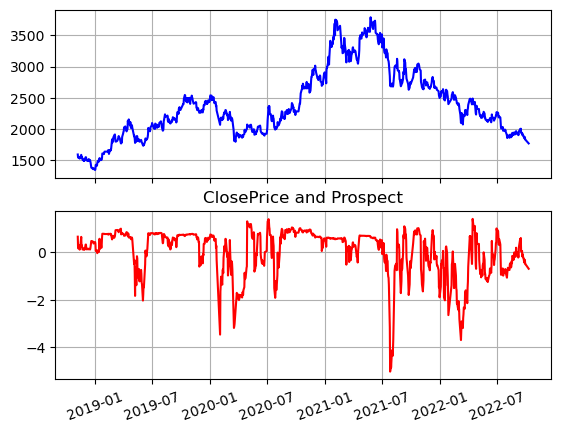
\includegraphics{figure/prospect_index_000001}
	\caption{收盘价和标准化的指数(以000001.SZ为例)}
	\label{fig:prospect_index_000001}
\end{figure}

\chapter{实证检验结果}

\section{持续性分析}
一般地,一个横截面特征在时间序列上是否具有持续性是相当重要的特征。我们分别计算了滞后阶数分别为1至5的相关系数,如图\ref{fig:consistency}所示。

\begin{figure}[htbp]
	\centering
	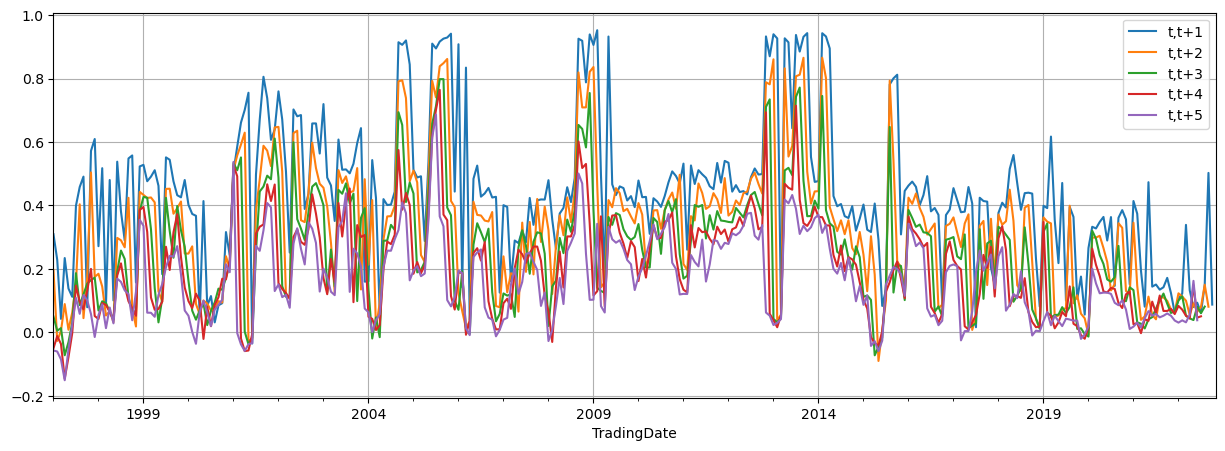
\includegraphics[scale=0.5]{figure/consistency}
	\caption{滞后阶数分别为1,2,3,4,5的横截面相关系数的时间序列线图}
	\label{fig:consistency}
\end{figure}

\section{组合分析}
首先,我们根据指数$PI$将样本按照20,40,60,80的样本内分位数分为5组,然后计算每一组的超额回报率;构造第五组和第一组的多空组合,并且观测其显著性。结果如表\ref{portfolio analysis}所示。


\begin{table}[htbp]
	\caption{多空组合分析结果}
	\label{portfolio analysis}
	\centering
	\begin{tabular}{@{}cccc@{}}
		\toprule
		变量名称          & 系数    & 标准差   & t统计量  \\ \midrule
		\multicolumn{4}{c}{简单平均}         \\ \midrule
		$PI_{mean}$     & 0.00094  &0.00061 & 1.53  \\
		$PI_{sum}$      & 0.000058 &0.00067& 0.09  \\ \midrule
		\multicolumn{4}{c}{流通市值加权平均}     \\ \midrule
		$PI_{mean}$ & -0.00078  &0.0018& -0.43 \\
		$PI_{sum}$  & 0.00069   &0.0018& 3.77  \\ \midrule
		\multicolumn{4}{c}{总市值加权平均}      \\ \midrule
		$PI_{mean}$   & -0.00039  &0.0018& -0.22 \\
		$PI_{sum}$  & 0.0061  &0.0018& 3.46  \\ \bottomrule
	\end{tabular}
\end{table}

\chapter{研究结论}
本文基于理论构建了针对个股的指数,对其持续性、预测能力等进行了检验,最后构建了相应的投资策略。本文构建的指数构造自1977年1月1日到2022年11月4日的A股日度股票数据,每一个股票在每一个时间点上均具有特异的指数,这为投资组合的分析创造了可行条件。

%---------------------------------------------------------------------
%  参考文献
%---------------------------------------------------------------------

\nocite{*}
{\color{black} \printbibliography}

\end{document}


